% Paper-ready section.  Compile from the codex_results directory.
% Required packages:
%   \usepackage{amsmath,amssymb,booktabs,graphicx,algorithm,algpseudocode}
% Optional for tighter float placement:
%   \usepackage[section]{placeins}

\section{Unknown-Distribution, Unknown-Cost Pandora Stopping}
\label{sec:pandora-algorithms}

\subsection{Problem definition}

For one prompt or programming problem, consider an exchangeable stream of
candidate generations (the ``boxes'').  Opening box $j$ reveals a raw score
$R_j$ and its character length $C_j$.  Before opening it, neither realization
is known.  More strongly, the prompt-specific reward law and the distribution
of the next character length are unknown.  After $n$ openings the observable
history and decision-space incumbent are
\begin{equation}
  \mathcal H_n=\{(R_j,C_j):j\le n\},
  \qquad
  V_n=\max_{j\le n}u_n(R_j),
\end{equation}
where $u_n$ converts a raw score into the policy's estimate of utility.  Let
$\mathcal U_x(j)$ denote the actual evaluation utility of candidate $j$ for
task $x$ (BT quality in alignment and binary correctness in coding).  Given a
character-cost divisor $D$, the evaluation objective is
\begin{equation}
  \mathbb E\!\left[
    \mathcal U_x(J_\tau)-\frac{1}{D}\sum_{j=1}^{\tau}C_j
  \right],
  \label{eq:pandora-objective}
\end{equation}
where $\tau$ is a stopping time and $J_\tau$ is the selected opened candidate.
Thus $1/D$ is the externally specified price of one character in utility
units; it is not the unknown quantity.  The unknown cost is the length of the
next generation.  Larger $D$ makes characters cheaper and normally induces
more openings.

For a known, homogeneous value law $F$ and known constant opening cost $c$,
classical Pandora stopping can be written in expected-improvement form:
continue from incumbent $v$ exactly when
\begin{equation}
  \mathbb E_{X\sim F}\big[(u(X)-v)_+\big]>c.
  \label{eq:known-pandora}
\end{equation}
Equivalently, the reservation value $z$ solves
$\mathbb E[(u(X)-z)_+]=c$.  Our setting replaces both sides of
Eq.~\eqref{eq:known-pandora}: an optimistic or regularized upper-tail model is
fit from training data and the opened prefix, and the next character cost is
estimated from the same information.  Because all future generations from a
given generator are treated as exchangeable, there is no ordering problem
among heterogeneous boxes; the decision is only whether to open one more.

\subsection{Utility--cost calibration}
\label{sec:utility-cost-calibration}

The raw reward and the character count cannot be compared directly.  The two
implementations put them into common units in two steps:
\begin{enumerate}
  \item \emph{Value calibration} maps the raw reward into an interpretable
  utility.  Alignment uses a Bradley--Terry (BT) probability of beating an
  online-estimated high-quality benchmark.  Coding uses an isotonic estimate
  of the probability that a program is correct.
  \item \emph{Cost calibration} divides the estimated next character count by
  $D$.  The stopping comparison is therefore ``expected utility improvement''
  versus ``expected character cost in utility units.''  The realized total
  cost reported by every experiment is the exact sum of the lengths actually
  opened, not this estimate.
\end{enumerate}

The phrase \emph{held-out calibration} requires care.  In coding, the isotonic
map is fit on all examples from the outer-training problems and then frozen;
it is held out from the final outer test, but it is not refit inside each fold
of the four-fold policy-selection calculation.  In alignment, no labeled
held-out utility map is fit: the BT benchmark is recomputed from the currently
opened prefix.  A full-pool benchmark is used only to score a stopped policy
after the fact and never enters its decisions.  Consequently, the claim that
the two value transforms are ``held-out calibration and BT'' is correct at a
high level only with these qualifications.

\subsection{A shared high-level algorithm}

Let $\widehat F_n^+$ be the fitted optimistic law of a future value, let
$\widehat C_n$ be the fitted mean length of the next generation, and let
$A_n$ and $B_n$ denote method-specific multiplicative and additive
regularizers.  Both implementations instantiate Algorithm~\ref{alg:blueprint}.

\begin{algorithm}[t]
\caption{Unknown-distribution, unknown-cost Pandora blueprint}
\label{alg:blueprint}
\begin{algorithmic}[1]
\Require Training data $\mathcal A$; divisor $D$; minimum openings $n_0$;
         horizon $H$
\State Fit a value map (if needed) and distribution/cost priors using only
       authorized pre-test data $\mathcal A$
\State Open $n_0$ candidates and observe their scores and exact lengths
\State $n\gets n_0$
\While{$n<H$}
  \State From $\mathcal H_n$, construct $u_n$, $\widehat F_n^+$, and
         $\widehat C_n$
  \State $V_n\gets\max_{j\le n}u_n(R_j)$
  \State $\widehat{\mathrm{EI}}_n\gets
         \mathbb E_{X\sim\widehat F_n^+}[(u_n(X)-V_n)_+]$
  \State $G_n\gets A_n\widehat{\mathrm{EI}}_n+B_n$
  \If{$G_n\le \widehat C_n/D$}
    \State \textbf{break}
  \EndIf
  \State Open candidate $n+1$; observe $(R_{n+1},C_{n+1})$; $n\gets n+1$
\EndWhile
\State \Return the incumbent opened candidate and charge
       $\sum_{j=1}^{n}C_j$ characters
\end{algorithmic}
\end{algorithm}

The stop inequality is non-anticipating: although the experiment code
vectorizes calculations over all prefixes, the entry used at prefix $n$
depends only on the first $n$ scores and lengths.  The implementation models
the reward tail and mean next length separately; it does not estimate or
exploit their joint dependence.

\subsection{Alignment instantiation: exponentiated-tail UCB--Pandora with BT utility}
\label{sec:alignment-instantiation}

\paragraph{What is fit.}
Each generator contains 100 prompts with 960 generations per prompt.  Within
each of ten split IDs 30--39, 50 prompts are training prompts and 50 are test
prompts.  For training prompt $i$, transform every raw reward as
$Y_{ij}=\exp(\operatorname{clip}(R_{ij},-50,50))$ and compute
\begin{align}
  a_i &= Q_{0.5}(Y_{i1},\ldots,Y_{i,960}),\\
  s_i &= \max\!\left\{
    \operatorname{mean}_{j:Y_{ij}\ge a_i}Y_{ij}-a_i,\epsilon
  \right\},\\
  \rho &= \operatorname{median}_{i\in\mathcal A}
           \frac{s_i}{\max(a_i,\epsilon)}.
  \label{eq:alignment-prior}
\end{align}
Only the relative tail-scale prior $\rho$ in
Eq.~\eqref{eq:alignment-prior} affects the retained policy.  Other stored
prior fields are inactive under the retained settings and are intentionally
omitted.  The policy configuration itself was frozen before these evaluated
splits:
\begin{equation}
 q=0.5,\quad \kappa_r=5,\quad \kappa_c=0,\quad
 \alpha=0.4,\quad \delta=0.05,\quad \eta=0.002,
 \quad n_0=3.
 \label{eq:alignment-config}
\end{equation}
Here and below, $\epsilon=10^{-8}$.

\paragraph{Online fit and utility.}
At prefix $n$, let $T_n$ contain the largest
$m_n=n-\lceil qn\rceil+1$ values among $Y_1,\ldots,Y_n$.  The inclusive
threshold convention is deliberate.  Define
\begin{align}
  \ell_n&=\min T_n,
  &\widetilde s_n&=\max\{\operatorname{mean}(T_n)-\ell_n,\epsilon\},\\
  s_n&=\frac{m_n\widetilde s_n+\kappa_r\ell_n\rho}{m_n+\kappa_r},
  &h_n&=\sqrt{\frac{\log(1/\delta)}{m_n}},\\
  s_n^+&=s_n(1+\alpha h_n),
  &s_n^-&=\max\{s_n(1-\alpha h_n),\epsilon\}.
  \label{eq:alignment-tail}
\end{align}
The fitted future upper tail has mass $1-q=0.5$ and
$Y=\ell_n+s_n^+Z$ for $Z\sim\operatorname{Exp}(1)$.  The online proxy for the
raw-reward 99th percentile and its BT utility are
\begin{equation}
  b_n=\log\!\left(\ell_n+s_n^-\log 50\right),
  \qquad u_n(r)=\sigma(r-b_n),
  \qquad \sigma(t)=\frac{1}{1+e^{-t}}.
  \label{eq:alignment-bt}
\end{equation}
Thus $u_n(r)$ is the BT probability that reward $r$ beats the estimated
high-quality benchmark, not a probability calibrated from correctness labels.

The implementation approximates the tail expected improvement with 48 fixed
midpoint exponential quantiles.  For
$z_k=-\log(1-(k+1/2)/48)$, $k=0,\ldots,47$, and raw incumbent
$r_n^\star=\max_{j\le n}R_j$,
\begin{align}
  \widehat{\mathrm{EI}}_n
  &=\frac{0.5}{48}\sum_{k=0}^{47}
    \left[
      \sigma\!\left(\log(\ell_n+s_n^+z_k)-b_n\right)
      -\sigma(r_n^\star-b_n)
    \right]_+,\\
  G_n&=\min\!\left\{
    \widehat{\mathrm{EI}}_n+\eta
    \sqrt{\frac{\log(1/\delta)}{2n}},\,1
  \right\},
  &\widehat C_n&=\frac{1}{n}\sum_{j=1}^{n}C_j.
  \label{eq:alignment-ei}
\end{align}
The cost prior has zero weight, so $\widehat C_n$ is exactly the running mean
of opened character counts.  Algorithm~\ref{alg:alignment-exact} is the exact
retained stopping calculation.

\begin{algorithm}[t]
\caption{Alignment: retained exponentiated-tail UCB--Pandora policy}
\label{alg:alignment-exact}
\begin{algorithmic}[1]
\Require Frozen $\rho$ from Eq.~\eqref{eq:alignment-prior}; divisor $D$;
         at most 960 generations
\State Open the first three generations; set $n\gets3$
\While{$n<960$}
  \State $Y_j\gets\exp(\operatorname{clip}(R_j,-50,50))$ for $j\le n$
  \State Form $T_n$ from the largest $n-\lceil0.5n\rceil+1$ values
  \State Compute $(\ell_n,s_n^+,s_n^-)$ by Eq.~\eqref{eq:alignment-tail}
        with $(\kappa_r,\alpha,\delta)=(5,0.4,0.05)$
  \State Compute $b_n$, the 48-point $\widehat{\mathrm{EI}}_n$, $G_n$, and
         $\widehat C_n$ by Eqs.~\eqref{eq:alignment-bt}--\eqref{eq:alignment-ei}
  \If{$G_n\le \widehat C_n/D$}
    \State \textbf{break}
  \EndIf
  \State Open generation $n+1$ and observe $(R_{n+1},C_{n+1})$;
         $n\gets n+1$
\EndWhile
\State \Return the opened generation with largest raw reward and charge its
       prefix's exact character sum
\end{algorithmic}
\end{algorithm}

\paragraph{How alignment is evaluated.}
For evaluation only, prompt $i$ has benchmark
$b_i^\star=R_{i,(951)}$, the 951st smallest of its 960 rewards (the code's
fixed empirical 0.99-quantile convention), and stopped quality
\begin{equation}
  Q_i(r)=\sigma(r-b_i^\star).
  \label{eq:alignment-eval-quality}
\end{equation}
This full-pool quantity never enters Algorithm~\ref{alg:alignment-exact}; the
algorithm uses the prefix benchmark $b_n$ from Eq.~\eqref{eq:alignment-bt}.

\subsection{Coding instantiation: shifted exponential in calibrated probability space}
\label{sec:coding-instantiation}

The coding experiments retain 83 problems for which at least one of 512
generations is correct.  Each outer split contains 41 training problems and 42
test problems.

\paragraph{Train-only value calibration.}
For outer split $s$, one nondecreasing isotonic regression is fit directly to
all $41\times512$ raw-reward/correctness pairs:
\begin{equation}
  \widehat g_s
  =\operatorname{IsoReg}\{(R_{ij},Y_{ij}):i\in\mathcal A_s,
      j=1,\ldots,512\},
  \qquad P_{ij}=\widehat g_s(R_{ij})\in[0,1].
  \label{eq:isotonic}
\end{equation}
Here $Y_{ij}\in\{0,1\}$ denotes correctness.  Samples have equal weight;
there is no reward binning.  Predictions outside the training score range are
clipped to the endpoint probabilities.  The frozen map is applied to both
training and test rewards, and Pandora utility is simply $u(R)=\widehat g_s(R)$.
There is no BT transform in the retained coding results.

\paragraph{Distribution and character priors.}
For each prior-fitting problem $i$ and tail quantile $q$, define
\begin{align}
  \ell_{i,q}&=Q_q(P_{i1},\ldots,P_{i,512}),\\
  s_{i,q}&=\max\!\left\{
    \operatorname{mean}_{j:P_{ij}\ge\ell_{i,q}}(P_{ij}-\ell_{i,q}),
    \epsilon
  \right\}.
\end{align}
The prior parameters are equal-problem averages
\begin{equation}
  \bar\ell_q=\operatorname{mean}_i\ell_{i,q},\qquad
  \bar s_q=\operatorname{mean}_i s_{i,q},
  \qquad
  \bar C=\operatorname{mean}_{i,j}C_{ij}.
  \label{eq:coding-prior}
\end{equation}
During four-fold policy selection, Eq.~\eqref{eq:coding-prior} is refit on the
three fit folds; for final evaluation it is refit on all 41 outer-training
problems.  The isotonic map in Eq.~\eqref{eq:isotonic}, however, is fit once on
all 41 outer-training problems before those inner folds.  The final 42-problem
outer test remains untouched by every fit and selection decision.

\paragraph{Online tail fit.}
For an opened prefix $P_1,\ldots,P_n$, let
\begin{align}
  B_n&=\max_{j\le n}P_j,
  &\ell_n&=Q_q(P_1,\ldots,P_n),\\
  I_n&=\{j\le n:P_j\ge\ell_n\},
  &m_n&=|I_n|,\\
  s_n&=\max\!\left\{
    \frac{1}{m_n}\sum_{j\in I_n}(P_j-\ell_n),\epsilon
  \right\}.
\end{align}
Location and scale are shrunk asymmetrically toward the training prior:
\begin{align}
  \widetilde\ell_n&=\frac{n\ell_n+\kappa_r\bar\ell_q}{n+\kappa_r},
  &\widetilde s_n&=\frac{m_ns_n+\kappa_r\bar s_q}{m_n+\kappa_r},\\
  h_n&=\sqrt{\frac{\log(1/\delta)}{m_n}},
  &\ell_n^+&=\operatorname{clip}_{[0,1]}
     (\widetilde\ell_n+\alpha\widetilde s_nh_n),\\
  &&s_n^+&=\widetilde s_n(1+\alpha h_n).
  \label{eq:coding-ucb}
\end{align}
The future upper tail has fixed mass $1-q$.  Conditional on being in that
tail, $X_n$ follows a shifted exponential with location $\ell_n^+$ and scale
$s_n^+$, truncated and renormalized on $[\ell_n^+,1]$:
\begin{equation}
 f_n(x)=
 \frac{\exp(-(x-\ell_n^+)/s_n^+)}
 {s_n^+\{1-\exp[-(1-\ell_n^+)/s_n^+]\}},
 \qquad \ell_n^+\le x\le1.
 \label{eq:coding-tail-density}
\end{equation}
Consequently,
\begin{align}
  \widehat{\mathrm{EI}}_n
  &=(1-q)\int_{\ell_n^+}^{1}(x-B_n)_+f_n(x)\,dx,\\
  \widehat C_n&=
  \frac{\sum_{j=1}^{n}C_j+\kappa_c\bar C}{n+\kappa_c},
  &G_n&=\left(\frac n3\right)^{-\gamma}\widehat{\mathrm{EI}}_n.
  \label{eq:coding-ei}
\end{align}
The code evaluates the integral using 32-point Gauss--Legendre quadrature
through the inverse CDF of Eq.~\eqref{eq:coding-tail-density}.  Specifically,
if $(x_k,w_k)_{k=1}^{32}$ are the Gauss--Legendre nodes and normalized weights
on $[0,1]$, and
$M_n=1-\exp[-(1-\ell_n^+)/s_n^+]$, the computed value is
\begin{equation}
 \widehat{\mathrm{EI}}_n=(1-q)\sum_{k=1}^{32}w_k
 \left[\ell_n^+-s_n^+\log(1-M_nx_k)-B_n\right]_+.
 \label{eq:coding-quadrature}
\end{equation}
At $\ell_n^+=1$ the conditional law is interpreted as a point mass at one.
Its tail mass remains exactly $1-q$ even when isotonic plateaus make $m_n$
larger than $(1-q)n$.

\begin{algorithm}[t]
\caption{Coding: shifted-exponential Pandora in correctness-probability space}
\label{alg:coding-exact}
\begin{algorithmic}[1]
\Require Frozen isotonic map $\widehat g_s$; prior
$(\bar\ell_q,\bar s_q,\bar C)$; parameters
$(q,\kappa_r,\kappa_c,\alpha,\gamma,\delta,D,H)$
\State Open three generations; observe $(R_j,C_j)$ and set
       $P_j\gets\widehat g_s(R_j)$ for $j=1,2,3$; $n\gets3$
\While{$n<H$}
  \State Compute $B_n$, the local tail statistics, and
         $(\ell_n^+,s_n^+)$ by Eq.~\eqref{eq:coding-ucb}
  \State Compute $\widehat{\mathrm{EI}}_n$, $\widehat C_n$, and $G_n$ by
         Eqs.~\eqref{eq:coding-tail-density}--\eqref{eq:coding-ei}
  \If{$G_n\le \widehat C_n/D$}
    \State \textbf{break}
  \EndIf
  \State Open generation $n+1$; observe $(R_{n+1},C_{n+1})$
  \State $P_{n+1}\gets\widehat g_s(R_{n+1})$; $n\gets n+1$
\EndWhile
\State \Return the first opened generation attaining $\max_{j\le n}P_j$ and
       charge the exact prefix character sum
\end{algorithmic}
\end{algorithm}

Equation~\eqref{eq:coding-ucb} is optimistic only when $\alpha>0$.  If
$\alpha=0$, Algorithm~\ref{alg:coding-exact} is a prior-regularized plug-in
Pandora rule, not a UCB rule.  The multiplier $(n/3)^{-\gamma}$ and the optional
horizon $H<512$ are empirical regularizers rather than parts of classical
Pandora stopping.  Isotonic plateaus can tie several candidates; the retained
implementation returns the first one attaining the maximum calibrated
probability.

\begin{table}[t]
\centering
\small
\caption{Exact instantiations of the shared blueprint.  ``Prefix'' means that
the quantity is recomputed using only opened candidates.}
\label{tab:pandora-instantiations}
\begin{tabular}{p{0.22\linewidth}p{0.35\linewidth}p{0.35\linewidth}}
\toprule
Component & Alignment & Coding \\
\midrule
Tail-model space & $\exp(R)$, unbounded shifted-exponential upper tail
& $\widehat g_s(R)\in[0,1]$, shifted-exponential upper tail truncated at 1 \\
Decision utility & Prefix BT probability $\sigma(R-b_n)$
& Frozen isotonic correctness probability $\widehat g_s(R)$ \\
Active training fit & Median tail scale/location ratio $\rho$
& Isotonic map, tail location/scale priors, and mean characters \\
Optimism & Upper tail scale, lower benchmark scale, plus an EI bonus
& Optional upper location and scale controlled by $\alpha$ \\
Next-cost estimate & Mean characters in the opened prefix ($\kappa_c=0$)
& Prefix/prior shrinkage with $\kappa_c\in\{0,10\}$ \\
EI regularizer & Additive confidence bonus
& Multiplicative $(n/3)^{-\gamma}$ tail decay \\
Hard horizon & 960, the available pool
& 512 or a training-chosen cap in the utility experiment; 512 for targets \\
\bottomrule
\end{tabular}
\end{table}

\subsection{What each experiment measures}
\label{sec:pandora-experiments}

\subsubsection{Alignment experiments}

The five alignment generators are Gemma-2-9B, Llama-3.1-8B,
Llama-3.2-3B, Mistral-7B, and Qwen-2.5-7B.  Each split uses four randomized
training permutations and eight randomized test permutations per prompt.
The three experiments reuse the same stopped prefixes but answer different
questions:
\begin{enumerate}
  \item \textbf{Utility objective.}  At each reported divisor
  $D\in\{10^5,5\!\times\!10^5,10^6,5\!\times\!10^6,10^7,5\!\times\!10^7\}$,
  training data choose the integer $N$ maximizing
  $\operatorname{mean}(Q)-\operatorname{mean}(C)/D$.  That $N$ is frozen on
  test, and its utility is compared with Algorithm~\ref{alg:alignment-exact}.

  \item \textbf{Equal-character head-to-head.}  On an independent set of test
  permutations, a randomized mixture of two adjacent Fixed-$N$ policies is
  chosen so that its \emph{aggregate expected} character count exactly matches
  the adaptive mean.  The reported score is
  $\Pr(R_{\rm adaptive}>R_{\rm fixed})+\tfrac12\Pr(\text{tie})$.  Because the
  matching uses held-out outcomes, this is a descriptive equal-budget
  comparison, not a deployable selection rule.

  \item \textbf{Target quality.}  For requested BT qualities
  $0.30,0.35,\ldots,0.60$, training interpolation selects between adjacent
  divisors on an 11-point adaptive frontier; a parallel interpolation selects
  adjacent Fixed-$N$ values.  Both are frozen for test.  The main cost-saving
  curve then performs a second, post-hoc interpolation of the held-out
  Fixed-$N$ curve to the adaptive policy's achieved held-out quality.  This
  quality-matched baseline is an oracle used for description, whereas the
  separately recorded direct comparison to the train-selected Fixed-$N$ rule
  is deployable.  Twenty-eight of 350 split--target rows, almost all at target
  0.30, lie outside the training adaptive frontier and are clamped.
\end{enumerate}

Figure~\ref{fig:alignment-overview} shows the three questions side by side.
Across $D\le10^7$, relative utility gains range from 1.31\% to 15.19\% and all
25 generator--divisor confidence intervals are above zero.  At
$D=5\times10^7$ the gains are only 0.08--0.33\%, and three of five intervals
include zero.  Every equal-character head-to-head interval is above 0.5.
Quality-matched target savings range from 10.23\% to 37.52\%, with all reported
intervals above zero; these latter savings retain the oracle-matching caveat.

\begin{figure*}[t]
  \centering
  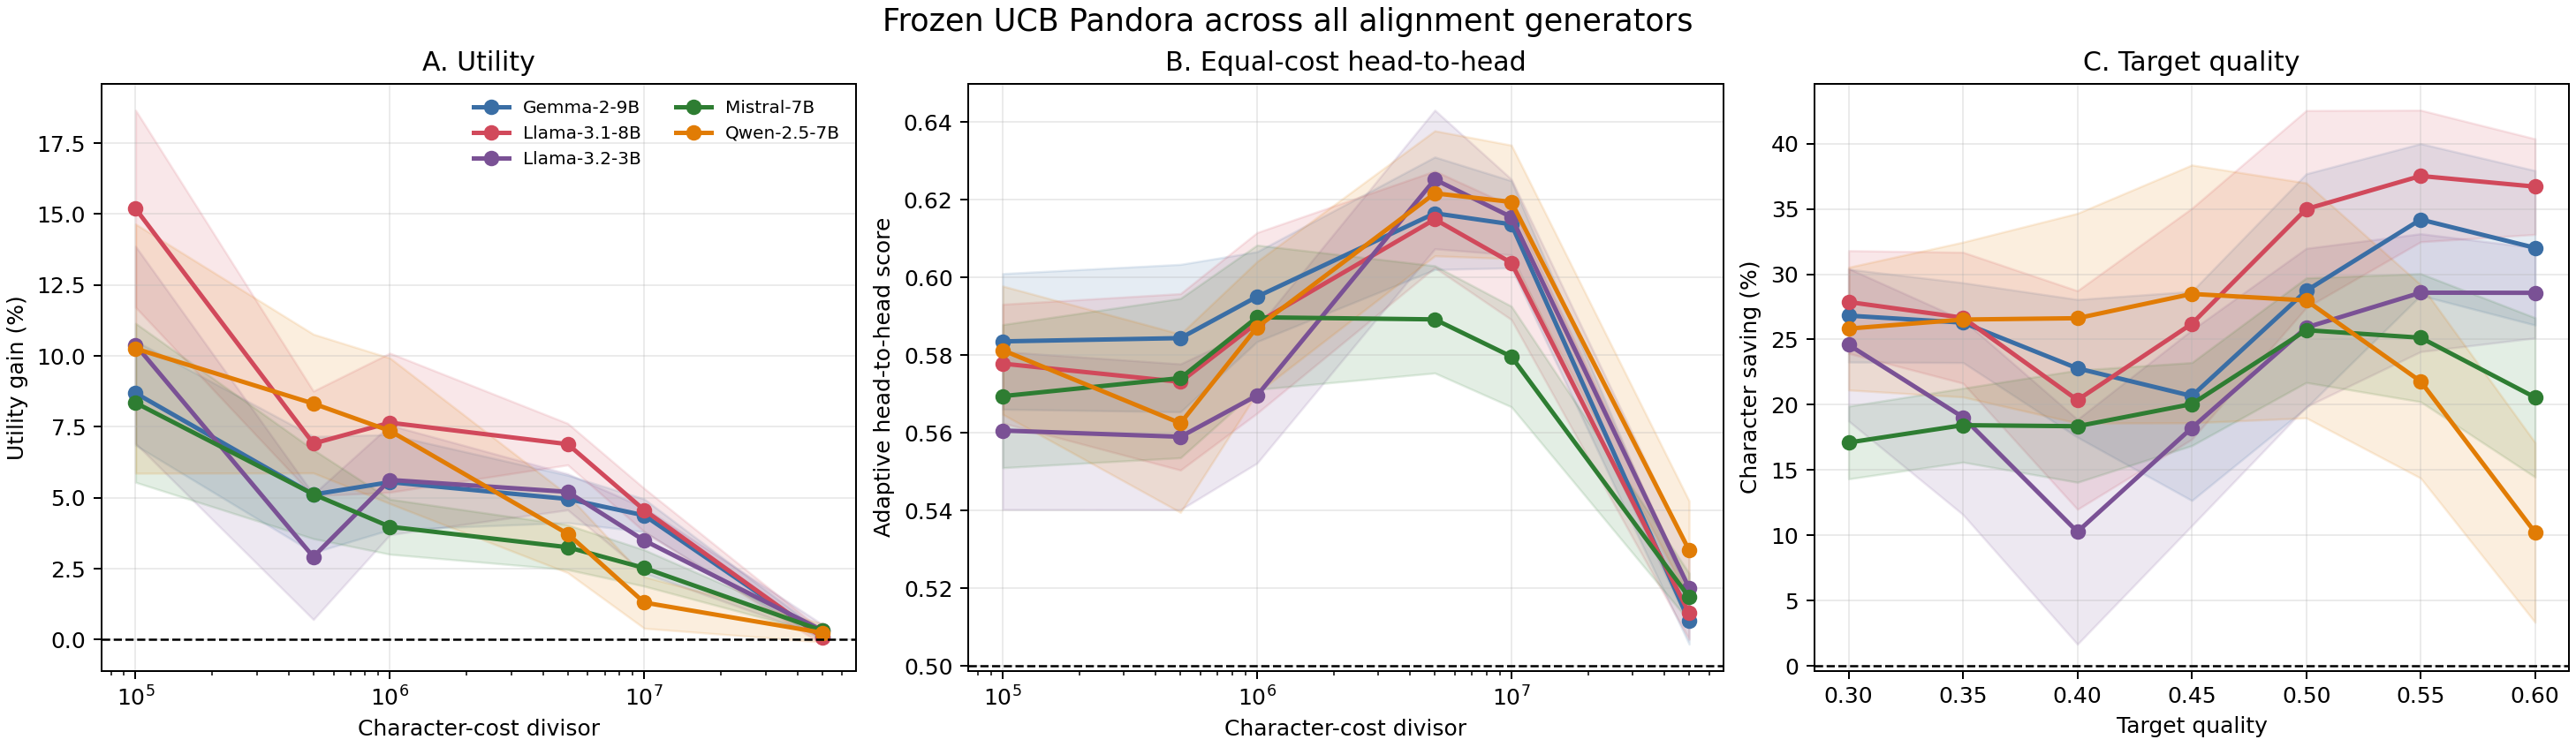
\includegraphics[width=0.98\textwidth]
    {results/alignment/all_generators_three_objectives.png}
  \caption{Alignment results over ten prompt splits for five generators.
  \textbf{A:} relative utility gain over the train-tuned, frozen Fixed-$N$
  policy.  \textbf{B:} raw-reward head-to-head score against an independent
  adjacent-$N$ mixture with exactly matched expected held-out characters;
  0.5 is parity.  \textbf{C:} character reduction relative to a post-hoc
  held-out Fixed-$N$ interpolation matched to achieved quality.  Bands are
  95\% Student-$t$ intervals over ten splits.  Panels B and C are controlled
  descriptive comparisons, not policy-selection procedures.}
  \label{fig:alignment-overview}
\end{figure*}

\subsubsection{Coding utility and equal-budget experiments}

For split IDs 75--84, each policy is tuned on 41 training problems using four
folds and four permutations per problem, then evaluated on 42 untouched test
problems with 48 permutations each.  For every divisor, selection is restricted
to the shifted-exponential family
\begin{equation}
 \begin{split}
 q&\in\{0.5,0.75\},\quad
 \alpha\in\{0,0.2,0.8\},\quad
 \kappa_r\in\{5,20,10^6\},\\
 \kappa_c&\in\{0,10\},\quad
 a\in\{1,1.1,1.2,1.3,1.5,2,\infty\},\quad \gamma=0.
 \end{split}
 \label{eq:coding-utility-grid}
\end{equation}
The selected configuration maximizes four-fold training utility
$\operatorname{accuracy}-\operatorname{characters}/D$.  If $a<\infty$, its
horizon is
\begin{equation}
 H=\min\{512,\max(3,\lceil aN_D^\star\rceil)\},
 \qquad
 N_D^\star=\arg\max_N
 \left\{A_{\rm train}(N)-\frac{N\bar C}{D}\right\};
 \label{eq:coding-cap}
\end{equation}
otherwise $H=512$.  Thus this experiment is not uniformly uncapped: 91 of the
100 saved split--divisor policies use a finite horizon.  Among the same 100
selections, 56 use $\alpha>0$ and 44 use $\alpha=0$.

The \emph{utility-gap} view compares test utility with the train-tuned,
frozen $N_D^\star$.  The \emph{equal-budget accuracy} view uses independent
test permutations and a post-hoc adjacent-$N$ mixture whose mean characters
exactly match the adaptive mean.  It isolates accuracy at a common measured
budget but is not deployable because the mixture is obtained from held-out
costs.  For example, at $D=10^5$ the shifted-exponential policy gains 5.75\%
utility (95\% CI 2.81--8.69\%) and 1.51 accuracy points at equal characters
(0.55--2.47).  At $D=3\times10^5$, the corresponding gains are 1.85\%
(0.09--3.61) and 0.73 points (0.17--1.28).  Most higher-divisor utility
intervals include zero, so the results do not support a claim of uniform gain
at every price.

\subsubsection{Coding target-quality experiment}

For final split IDs 95--104, four-fold selection uses 16 training
permutations per problem and final evaluation uses 48 test permutations per
problem.  Each target
$\tau\in\{0.25,0.30,0.35\}$ selects one uncapped shifted-exponential
configuration and one of 19 divisors.  The family grid is
\begin{equation}
 q\in\{0.5,0.75\},\quad
 \alpha\in\{0,0.2,0.8\},\quad
 \kappa_r\in\{5,20,10^6\},\quad
 \kappa_c\in\{0,10\},\quad
 \gamma\in\{0,0.25,0.5,1\},\quad H=512.
 \label{eq:coding-target-grid}
\end{equation}
A frozen development profile is first built from held-out evaluations on
split IDs 55--59.  For policy $h$ and divisor $D$, it stores mean accuracy
$A_{\rm prof}(h,D)$ and geometric-mean characters
\begin{equation}
 C_{\rm prof}(h,D)=
 \exp\!\left\{\frac15\sum_{s=55}^{59}\log C_s(h,D)\right\}.
\end{equation}
On current outer split $s$, the feasibility score is
\begin{equation}
 A_{{\rm sel},s}(h,D)=0.1A_{{\rm CF},s}(h,D)+0.9A_{\rm prof}(h,D).
 \label{eq:coding-target-selection}
\end{equation}
Among candidates with $A_{{\rm sel},s}\ge\tau$, selection minimizes frozen
$C_{\rm prof}$, with smaller overshoot and then fixed identifiers breaking
ties.  Current-split character cost receives zero selection weight.  The
implementation has a cheapest-max-score fallback if no candidate is feasible,
but it was inactive because all 30 retained choices passed their selection
threshold.  There is no policy mixture, target margin, lower-confidence
threshold, Fixed-$N$ guard, or test-time selection.  All 30 selected policies
have $\gamma>0$; 27 have $\alpha>0$ and three have $\alpha=0$.

Two integer Fixed-$N$ baselines answer different questions.  The deployable
baseline is the cheapest training $N$ whose exact training accuracy reaches
$\tau$, frozen before test.  The descriptive oracle is the cheapest held-out
$N$ whose accuracy reaches the \emph{adaptive policy's achieved held-out
accuracy}.  Mean achieved accuracies for requested targets 0.25, 0.30, and
0.35 are 0.2503, 0.2923, and 0.3448, respectively.  The respective character
savings against the held-out matched oracle are 33.86\%, 28.06\%, and 35.69\%;
the last 95\% interval includes zero.  Per-split target hit rates are 5/10,
3/10, and 3/10, so the procedure tracks targets in aggregate but does not
guarantee that every held-out split reaches them.

\begin{figure*}[t]
  \centering
  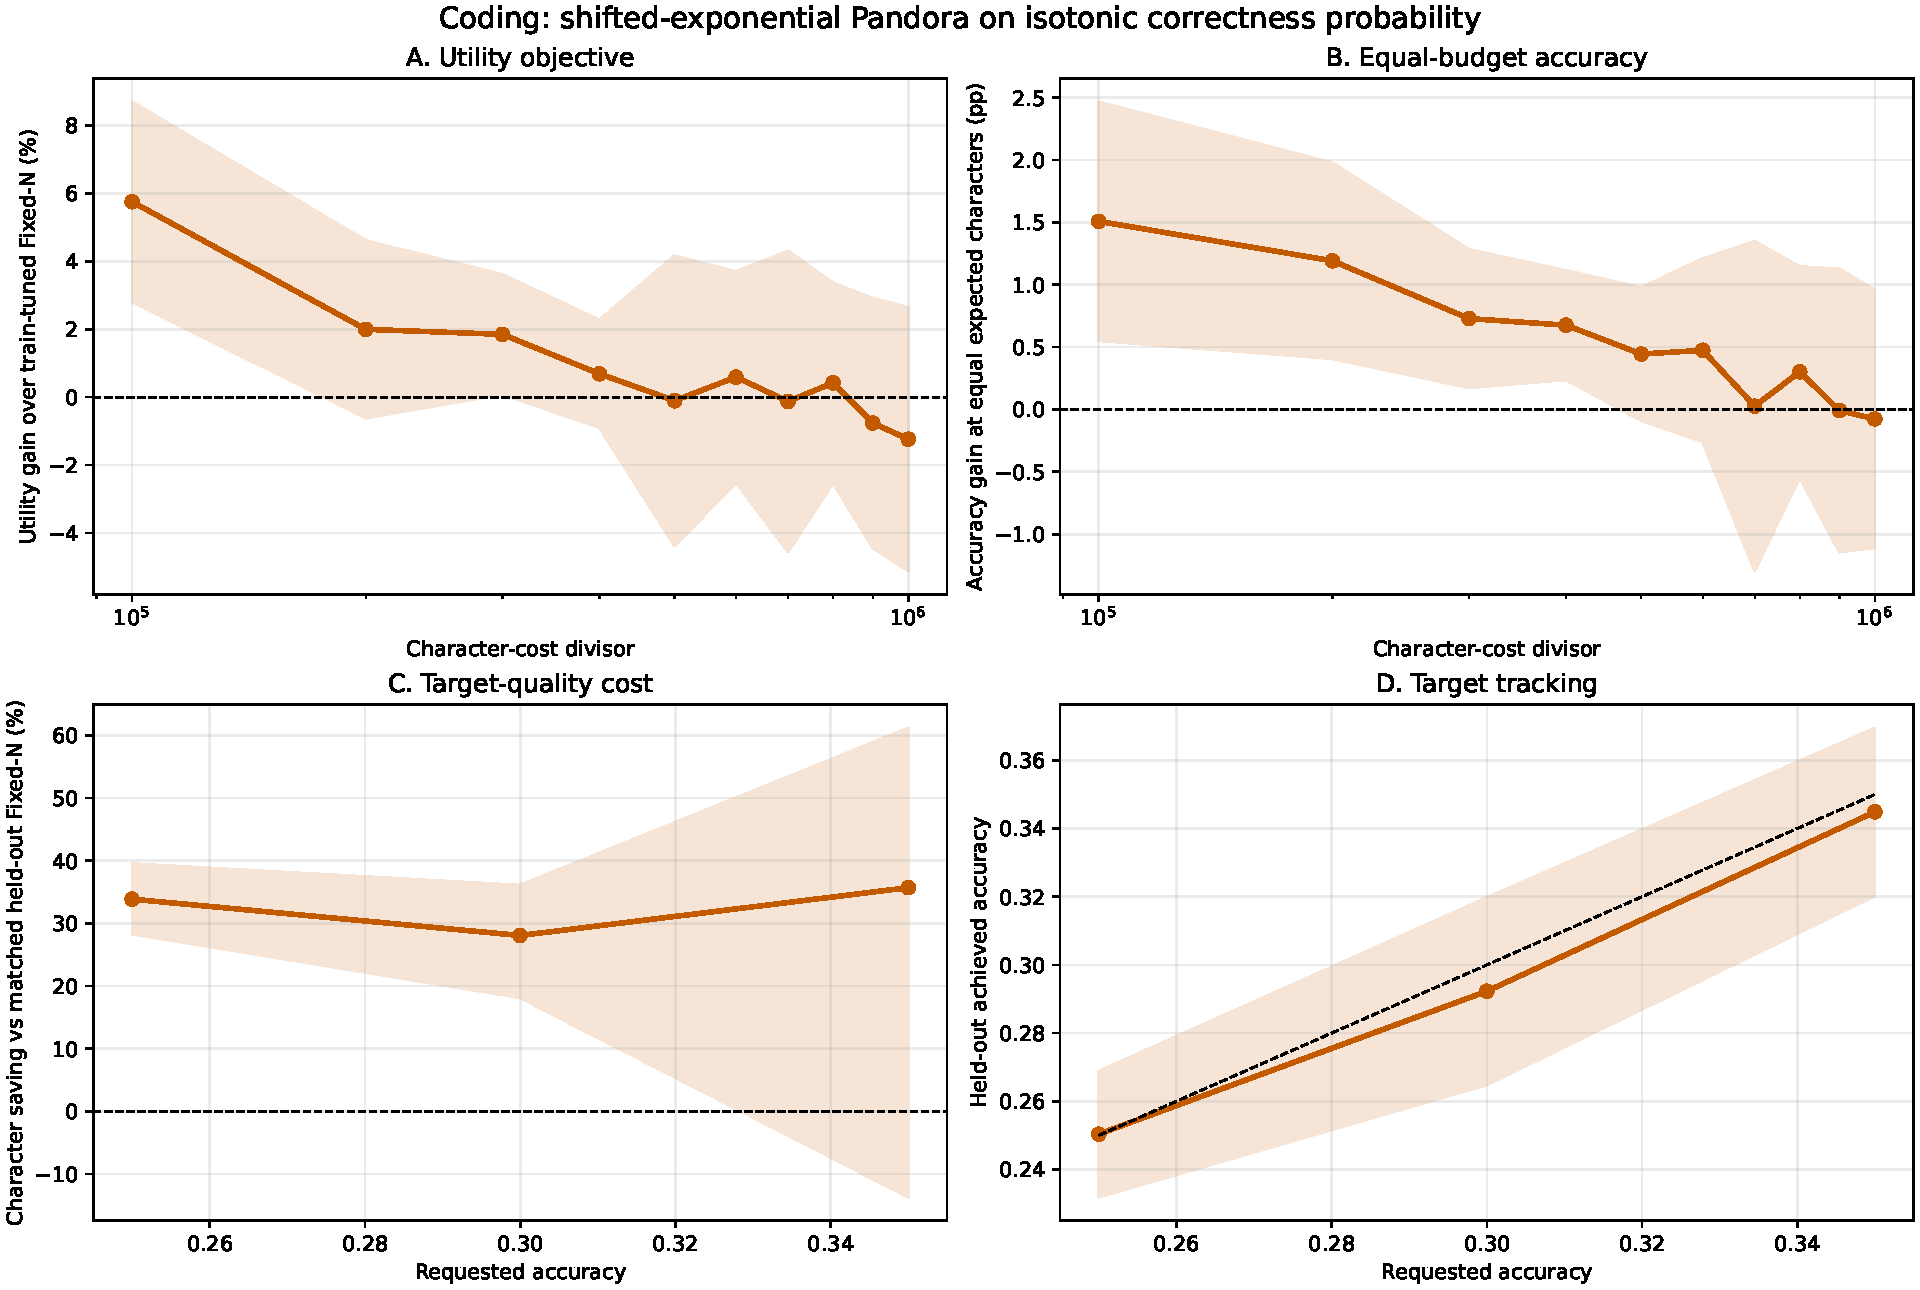
\includegraphics[width=0.88\textwidth]
    {results/algorithm_section/coding_shifted_exponential_overview.pdf}
  \caption{Coding results for the shifted-exponential calibrated-probability
  family only.  \textbf{A:} relative test-utility gain over train-tuned
  Fixed-$N$.  \textbf{B:} test-accuracy gain against a post-hoc adjacent-$N$
  mixture with exactly matched expected characters.  \textbf{C:} target-mode
  character savings against a post-hoc held-out Fixed-$N$ matched to achieved
  accuracy.  \textbf{D:} achieved versus requested accuracy; the diagonal is
  exact target tracking.  Utility/equal-budget and accuracy bands are 95\%
  Student-$t$ intervals over ten splits; panel C uses a paired split bootstrap.
  Panels B and C are descriptive oracle matches, while panels A and D evaluate
  policies selected without final-test outcomes.}
  \label{fig:coding-overview}
\end{figure*}

\subsection{Relation to unknown-distribution, unknown-cost Pandora's box}
\label{sec:pandora-relation}

Both systems are faithful instantiations of the same empirical Pandora
blueprint: opening a generation reveals an initially unknown value and an
initially unknown character cost; a training-regularized tail law estimates
the value of one more opening; an online mean estimates its cost; and the
policy stops when adjusted expected improvement no longer pays for that cost.
Alignment instantiates the blueprint with a genuinely optimistic
exponentiated tail and a dynamic BT utility.  Coding instantiates it with a
bounded shifted-exponential tail after a frozen isotonic utility transform,
plus optional optimism, optional character shrinkage, tail decay, and—in the
utility experiment—often a training-derived hard horizon.

Accordingly, \emph{unknown-distribution, unknown-cost Pandora policy} is the
accurate umbrella description.  \emph{UCB--Pandora} is accurate for the
alignment rule and for coding configurations with $\alpha>0$, but not for
coding configurations with $\alpha=0$.  These are empirical reservation
policies, not claims of Weitzman-optimal behavior: the tail model can be
misspecified, cost uses only a marginal mean, coding adds empirical
regularizers, and finite pools sampled without replacement impose hard
horizons.  These qualifications identify each instantiation without changing
the blueprint in Algorithm~\ref{alg:blueprint}.
